\chapter{Sequence models}

Next, we will implement models which take the ordering of tokens into
account. This includes \acp{CNN} and \acp{RNN}.

For the models in this chapter, we needed to set a fixed number of tokens
such that shorter documents were padded to this length, and longer documents
truncated. In order to decide this, we examined the distribution of document
lengths in the training set. All subsequent values are rounded to the nearest
integer. First, we found the 95th percentile of document lengths, which
turned out to be 701 tokens. Then, we computed the value $Q_2 + 1.5 \cdot
(Q_3 - Q_1)$, or the median plus 1.5 times the interquartile range, which
gives 693 tokens. Finally, we computed the mean value plus two standard
deviations, giving 707 tokens. These values are all close to each other, and
we decided to settle on 700 tokens since it is a round number close to all
values we examined.


\section{Convolutional neural networks}

We create a model with convolutional architecture based on the model
described in \textcite{zhang2017sensitivity}. The basis of this architecture
is a set of filter banks with varying window size. After applying the
convolutions, the output is pooled along the time axis, leaving a vector with
as many elements as there are filters in the filter banks. The vectors for
each of the filter banks are concatenated into a single vector.


\subsection{Results}

The \ac{CNN} classifier that used both tokens and POS tags as input performed
better than the one which only used tokens as input, as seen in table
\ref{tab:cnn-results}. However, on the collapsed label set, the model which only
used tokens had a higher accuracy. Filters of size 4, 5, and 6 were used.

\begin{table}
  \centering
  \begin{tabular}{lrrrr}
    \toprule
            & \multicolumn{2}{c}{All labels} & \multicolumn{2}{c}{Collapsed labels} \\
    \cmidrule(lr){2-3}
    \cmidrule(lr){4-5}
    Model     & Macro \FI      & Micro \FI      & Macro \FI      & Micro \FI \\
    \midrule
    Tokens    &         $0.234$  &         $0.415$  &         $0.423$  & $\mathbf{0.797}$ \\
    +POS      & $\mathbf{0.283}$ &         $0.431$  & $\mathbf{0.444}$ &         $0.772$  \\
    %           cnn-02-11_14-52-21                    cnn-02-11_15-00-41
    Mixed POS &         $0.276$  & $\mathbf{0.472}$ &         $0.423$  & $\mathbf{0.797}$ \\
    % Windows 2, 3, 4
    %           cnn-02-11_15-15-08                    cnn-02-13_12-11-43
    Mixed POS &         $0.265$  &         $0.455$  &         $0.430$  &         $0.748$  \\
    \midrule
    % pre-trained embeddings, windows 2,3,4. Max pooling only
    %           cnn-02-13_14-41-37
    +POS      &         $0.259$  &         $0.447$  &         $0.388$  &         $0.732$  \\
    \bottomrule
  \end{tabular}
  \caption{\FI scores of CNN classifiers on AES}
  \label{tab:cnn-results}
\end{table}


\section{Recurrent neural networks}

A \ac{LSTM} \ac{RNN} was implemented based on the architecture described by
\textcite{taghipour16}. Several changes to their architecture were made in
order to accomodate our data. For instance, \citeauthor{taghipour16} modelled
the task as a regression problem, their output layer consisting of a single
node with a value constrained to (0, 1) by the sigmoid function. This layer
was replaced with a softmax layer similar to the \acp{MLP} in section
\ref{subsec:mlp}.

We then chose a loss function to be compatible with a multi-class softmax
output. We used categorical cross-entropy. A different evaluation metric was
also needed because we are treating the task as multi-class prediction. We
are reporting macro and micro \FI as before. The \ac{QWK} metric used by
\citeauthor{taghipour16} is not applicable to the predictions of our
classifier.

The formulation of the \ac{AES} task as a regression problem by \citeauthor{taghipour16}
was partly a constraint stemming from the Kaggle competition that supplied
the data and problem formulation, and partly motivated by the nature of the
data. The ASAP data consists of essays from eight different prompts, and the
scoring methods differs across prompts. Since the scores are numeric values over
different ranges, modelling the task as a regression problem made it sufficient
to normalize the numeric scores to a common interval before training.

Generally for \ac{AES}, modelling the task as multi-class prediction is common,
and is used in \autocite{vajjala18universalCEFR}. In \autocite{vajjala17}, two
different datasets with different properties were used, and the author utilized
both multi-class prediction and regression at different points.

The embedding layer in \textcite{taghipour16} was initialized with
pre-trained embeddings of size 50. Our embedding layer was initialized to
random vectors and trained as part of the network.

Unlike our corpus, ASK, the dataset used by \citeauthor{taghipour16}
contained essays that were not necessarily written in a second language. Our
data is not split into different parts based on the prompt. There are two
different test levels in ASK, but these are not distinguished in training.

Note that the activation function for the gates in gated RNNs in Keras by
default is the \emph{Hard sigmoid} activation function (ref. eq.
\ref{eq:hardsigmoid}), chosen because it is computationally more efficient
than the sigmoid function.

We also experimented with a different type of gated \ac{RNN} cell, the
\ac{GRU}. This variant of \ac{RNN} is slightly simpler than the \ac{LSTM},
featuring only two gates. However, it is still designed to be able to
propagate the error gradient over a larger number of timesteps and is
supposed to solve the same problems as \ac{LSTM}. The equations defining
\ac{LSTM} \ac{GRU} cells are listed in chapter \ref{ch:background}, equations
\ref{eq:lstm} and \ref{eq:gru}.


\subsection{Variants}

We attempt two different methods of combining the sequence of hidden states
from the \ac{RNN} into a feature vector. The simplest approach is \emph{mean
over time}, where we use the elementwise average of elements in hidden states
across the time dimension as our feature vector. The mean over time layer is
used in two of the experiments. Once with a \ac{RNN} processing the essay
from top to bottom, and once on top of a bidirectional RNN.

The bidirectional model (BiRNN) is constructed by running two \acp{RNN} over
the same input, but in the opposite order. The output from the BiRNN layer is
a sequence of vectors where, for each timestep $j$, the vector is the
concatenation of two vectors $[s_f;s_b]$ where $s_f$ at timestep $j$ is the
output from the forwards \ac{RNN} after processing the inputs $(x_1, x_2,
\ldots, x_j)$ and $s_b$ the output from the backwards \ac{RNN} after
processing the inputs $(x_m, x_{m-1}, \ldots, x_j)$, $m$ being the total
number of timesteps. The BiRNN should therefore be able to extract context on
both sides of a input timestep.

\todo{Mean of the final state}
\todo{Add POS inputs to RNN}
\todo{GRU cells}

The attention model uses an attention layer, which instead computes a
weighted sum of the states, and therefore should be able in theory to
disregard uninformative timesteps and improve performance. In order to find
the weight to apply to each state, a single-layer neural network computes a
value between -1 and 1 for each timestep. These values are normalized by a
softmax layer and then used to compute the weighted average. The attention
mechanism is trained along with the rest of the network. The attention models
use unidirectional \acp{RNN}.

All the models a hidden state vector of size 300 in the \ac{RNN}. The
vocabulary was limited to the 4,000 most common words.


\subsection{Results}

Results for four different models are shown in table \ref{tab:rnn-results}. All
but \emph{Modified} are using the same hyperparameters as
\citeauthor{taghipour16}. The \emph{Attention} model does not use masking,
while \emph{Mean/Time} and \emph{BiLSTM} do.
\todo{Always use pre-trained embeddings when repeating the experiments?}

\begin{table}
  \centering
  \begin{tabular}{lrrrr}
    \toprule
            & \multicolumn{2}{c}{All labels} & \multicolumn{2}{c}{Collapsed labels} \\
    \cmidrule(lr){2-3}
    \cmidrule(lr){4-5}
    Model     & Macro \FI      & Micro \FI      & Macro \FI      & Micro \FI \\
    \midrule
              \multicolumn{5}{c}{50 dimensional, randomly initialized embeddings} \\
    \midrule
    % 50 dim, random init
    %           taghipour_ng-2019-01-15_20-50-06      taghipour_ng-2019-01-15_20-46-42
    Mean/Time &         $0.280$  &         $0.382$  &         $0.461$  &         $0.699$  \\
    %           taghipour_ng-2019-01-22_12-58-00      taghipour_ng-2019-01-22_13-01-44
    BiLSTM    &         $0.286$  &         $0.398$  &         $0.485$  &         $0.683$  \\
    %           rnn-25832764                          rnn-25832765
    Attention &         $0.244$  & $\mathbf{0.423}$ & $\mathbf{0.559}$ &         $0.780$  \\
    \midrule
    % 50 dim, pretrained, fine tune
              \multicolumn{5}{c}{50 dimensional, pre-trained embeddings, w/ fine tuning} \\
    \midrule
    %           rnn-25832746                          rnn-25832747
    Mean/Time &         $0.285$  &         $0.415$  &         $0.466$  &         $0.659$  \\
    %           rnn-25832748                          rnn-25832749
    BiLSTM    &         $0.257$  &         $0.374$  &         $0.447$  &         $0.691$  \\
    %           taghipour_ng-2019-01-24_19-16-41      taghipour_ng-2019-01-24_21-23-34
    Attention &         $0.303$  &         $0.423$  &         $0.558$  & $\mathbf{0.805}$ \\
    \midrule
    % 100 dim, pretrained, fine tune
              \multicolumn{5}{c}{100 dimensional, pre-trained embeddings, w/ fine tuning} \\
    \midrule
    %           rnn-25832716                          rnn-25832717
    Mean/Time &         $0.271$  &         $0.390$  &         $0.496$  &         $0.724$  \\
    %           rnn-25831870                          rnn-25831871
    BiLSTM    &         $0.301$  &         $0.350$  &         $0.456$  &         $0.683$  \\
    %           rnn-25832718                          rnn-25832719
    Attention &         $0.288$  &         $0.398$  &         $0.538$  &         $0.797$  \\
    \midrule
    % GRU cells, attention
              \multicolumn{5}{c}{GRU cells with attention} \\
    \midrule
    %           rnn-25858207                          rnn-25858208
    Rnd. init &         $0.299$  &         $0.431$  &         $0.533$  &         $0.764$  \\
    %           rnn-25858209                          rnn-25858211
    Pre train & $\mathbf{0.354}$ &         $0.390$  &         $0.493$  &         $0.724$  \\
    \midrule
    % LSTM cells, attention, frozen embeddings
              \multicolumn{5}{c}{LSTM + Attention with pre-trained, frozen embeddings} \\
    \midrule
    %           rnn-25858349                          rnn-25858350
    50 dim    &         $0.261$  & $\mathbf{0.488}$ &         $0.511$  &         $0.772$  \\
    %           rnn-25858483                          rnn-25858494
    100 dim   &         $0.271$  &         $0.472$  &         $0.491$  &         $0.707$  \\
    \bottomrule
  \end{tabular}
  \caption{\FI scores of RNN classifiers}
  \label{tab:rnn-results}
\end{table}

We find that the best performing models all use the attention mechanism.
Keep in mind that the stopping criterion is the macro \FI score, and thus
the micro \FI score is to be considered a side effect of the macro \FI.

\todo{Analysis of attention model}
\todo{Per-class results}


\section{Native language identification}

Unlike the proficiency labels in ASK, \ac{L1}s are rather evenly distributed.

We train the same models to classify the documents by native language. The
performance of a \ac{CNN} model improved drastically when including \ac{POS}
tags as input, as evident in table \ref{tab:cnn-nli-results}.

A RNN was able to outperform the CNN only slightly, and here it was not the
attention model that was best, but a bidirectional LSTM.

\begin{table}
  \centering
  \begin{tabular}{lrr}
    \toprule
    Model     & Macro \FI      & Micro \FI \\
    \midrule
    Tokens    &         $0.367$  &         $0.366$  \\ % cnn-nli-2019-02-05_12-54-51
    +POS      & $\mathbf{0.467}$ & $\mathbf{0.463}$ \\ % cnn-nli-2019-01-30_15-32-28
    \bottomrule
  \end{tabular}
  \caption{\FI scores of CNN classifiers on NLI}
  \label{tab:cnn-nli-results}
\end{table}

\begin{table}
  \centering
  \begin{tabular}{lrr}
    \toprule
    Model     & Macro \FI      & Micro \FI \\
    \midrule
    Mean/Time &         $0.379$  &         $0.390$  \\ % rnn_nli-25740792
    BiLSTM    & $\mathbf{0.468}$ & $\mathbf{0.480}$ \\ % rnn_nli-25740786
    Attention &         $0.423$  &         $0.407$  \\ % rnn_nli-25740789
    \bottomrule
  \end{tabular}
  \caption{\FI scores of RNN classifiers on NLI}
  \label{tab:rnn-nli-results}
\end{table}
\todo{Include POS in RNN models}

The attention model allows us to visualize the weights the network gives to
each token in a document. Figure \ref{fig:nli-attention} shows the first 300
tokens of a text which was correctly predicted to be written by a native Polish
speaker. Red tokens indicate timesteps that were given higher weight by the attention
model, and blue tokens ones that were given low weights. Out of vocabulary tokens
are replaced by question mark emoji. The attention values do not seem easily
interpretable, as there are lexical and grammatical errors both in the red and
the blue sections.

\begin{figure}
  \centering
  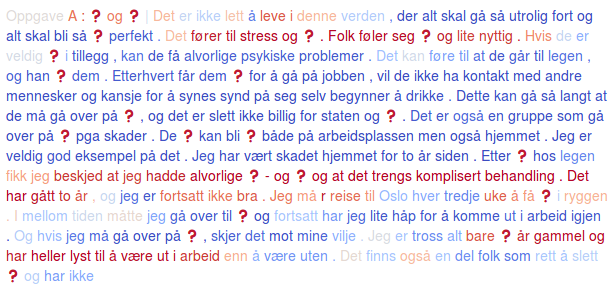
\includegraphics[width=\textwidth]{nli-attention}
  \caption{Attention values of NLI classifier on excerpt from ASK text h0131}
  \label{fig:nli-attention}
\end{figure}
